\documentclass[11pt,class=report,crop=false]{standalone}
\usepackage{exo7hilisit}

\begin{document}


\entete{Hilisit}{Capacité mathématiques}

\titre{\'Equations différentielles -- Partie 2 : Notion d'équation différentielle} 

\bigskip
\bigskip



%%%%%%%%%%%%%%%%%%%%%%%%%%%%%%%%%%%%%%%%%%%%%%%%%%%%%%%%%%%%
%\section{Notion d'équation différentielle}


\exercice{}
\enonce
Vérifier que les fonctions $f$ suivantes sont solutions de l'équation différentielle donnée.
\begin{enumerate}
  \item $f(x) = -e^{2x}$, $y'=2y$.
  \item $f(x) = \frac{1}{2-x}$, $y'=y^2$.
  \item $f(x) = (3+2x)e^x$, $y''-2y'+y=0$.
  \item $f(x) = Ce^{-x}+\sin(x)-\cos(x)$ (quelle que soit la constante $C$), $y'+y=2\sin(x)$
\end{enumerate} 
\finenonce

\indication
Il faut calculer la dérivée $f'(x)$ (et si besoin la dérivée seconde $f''(x)$) et vérifier que $f$ et $f'$ (et éventuellement $f''$) satisfont la relation donnée par l'équation différentielle (en remplaçant $y$ par $f$, $y'$ par $f'$...).
\finindication

\correction
\sauteligne
\begin{enumerate}
  \item $f(x) = -e^{2x}$, $f'(x) = -2e^{2x}$ donc on a bien $f'(x)=2f(x)$.
  \item $f(x) = \frac{1}{2-x}$, $f'(x) = \frac{1}{(2-x)^2}$ donc on a bien  $f'(x)=f(x)^2$.
  \item $f(x) = (3+2x)e^x$,  $f'(x) = (5+2x)e^x$, $f''(x) = (7+2x)e^x$ donc on a bien  $f''(x)-2f'(x)+f(x)=((3+2x) -2(5+2x)+(7+2x))e^x = 0\cdot e^x = 0$.
  \item $f(x) = Ce^{-x}+\sin(x)-\cos(x)$, $f'(x) = -Ce^{-x}+\cos(x)+\sin(x)$, donc on a bien  $f'(x)+f(x)=2\sin(x)$.
\end{enumerate} 
\fincorrection
\finexercice


\exercice{}
\enonce
Déterminer toutes les solutions constantes des équations différentielles suivantes.
\begin{enumerate}
  \item $y'+y=5$
  \item $y'=y^2-y$
  \item $y'=y^2-4y+1$
  \item $y' = y + x$
\end{enumerate} 
\finenonce

\indication
Si $f(x)=k$ est une fonction constante, alors $f'(x)=0$ pour tout $x$. Une des équations n'admet aucune solution constante !
\finindication

\correction
\sauteligne
 \begin{enumerate}
  \item Si $f$ est une fonction constante, alors $f(x)=k$ pour tout $x$, donc $f'(x)=0$ pour tout $x$. Si $f$ est solution de l'équation différentielle $y'+y=5$, alors $f'(x)+f(x)=5$ pour tout $x$, donc $0+k=5$, donc $k=5$. La seule solution constante est la solution $f(x)=5$ pour tout $x$.

  \item Si $f(x)=k$ est solution de l'équation différentielle $y'=y^2-y$, alors $f'(x)=f(x)^2-f(x)$ pour tout $x$, donc $0=k^2-k$, donc $k(k-1)=0$, donc $k=0$ ou $k=1$.
  Il y a deux solutions constantes  $f(x)=0$ pour tout $x$ (la fonction nulle) et $f(x)=1$ pour tout $x$.
  
  \item Si $f(x)=k$ est solution de l'équation différentielle $y'=y^2-4y+1$, alors $f'(x)=f(x)^2-4f(x)+1$, donc $0=k^2-4k+1$. Les solutions de $k^2-4k+1=0$ sont $k_1=2-\sqrt3$ et $k_2=2+\sqrt3$  qui définissent les deux solutions constantes.
  
  \item Si $f(x) = k$ est solution de l'équation différentielle $y'=y+x$, alors $f'(x) = f(x) + x$ donc $0 = k + x$ et alors $k=-x$. Ceci est une contradiction car $k$ doit être une constante (un nombre fixé !). Ainsi cette équation différentielle n'admet aucune solution constante.
\end{enumerate} 
\fincorrection
\finexercice


\exercice{}
\enonce

Le dessin représente quelques solutions de l'équation différentielle $y'=y-1$.

\begin{center}
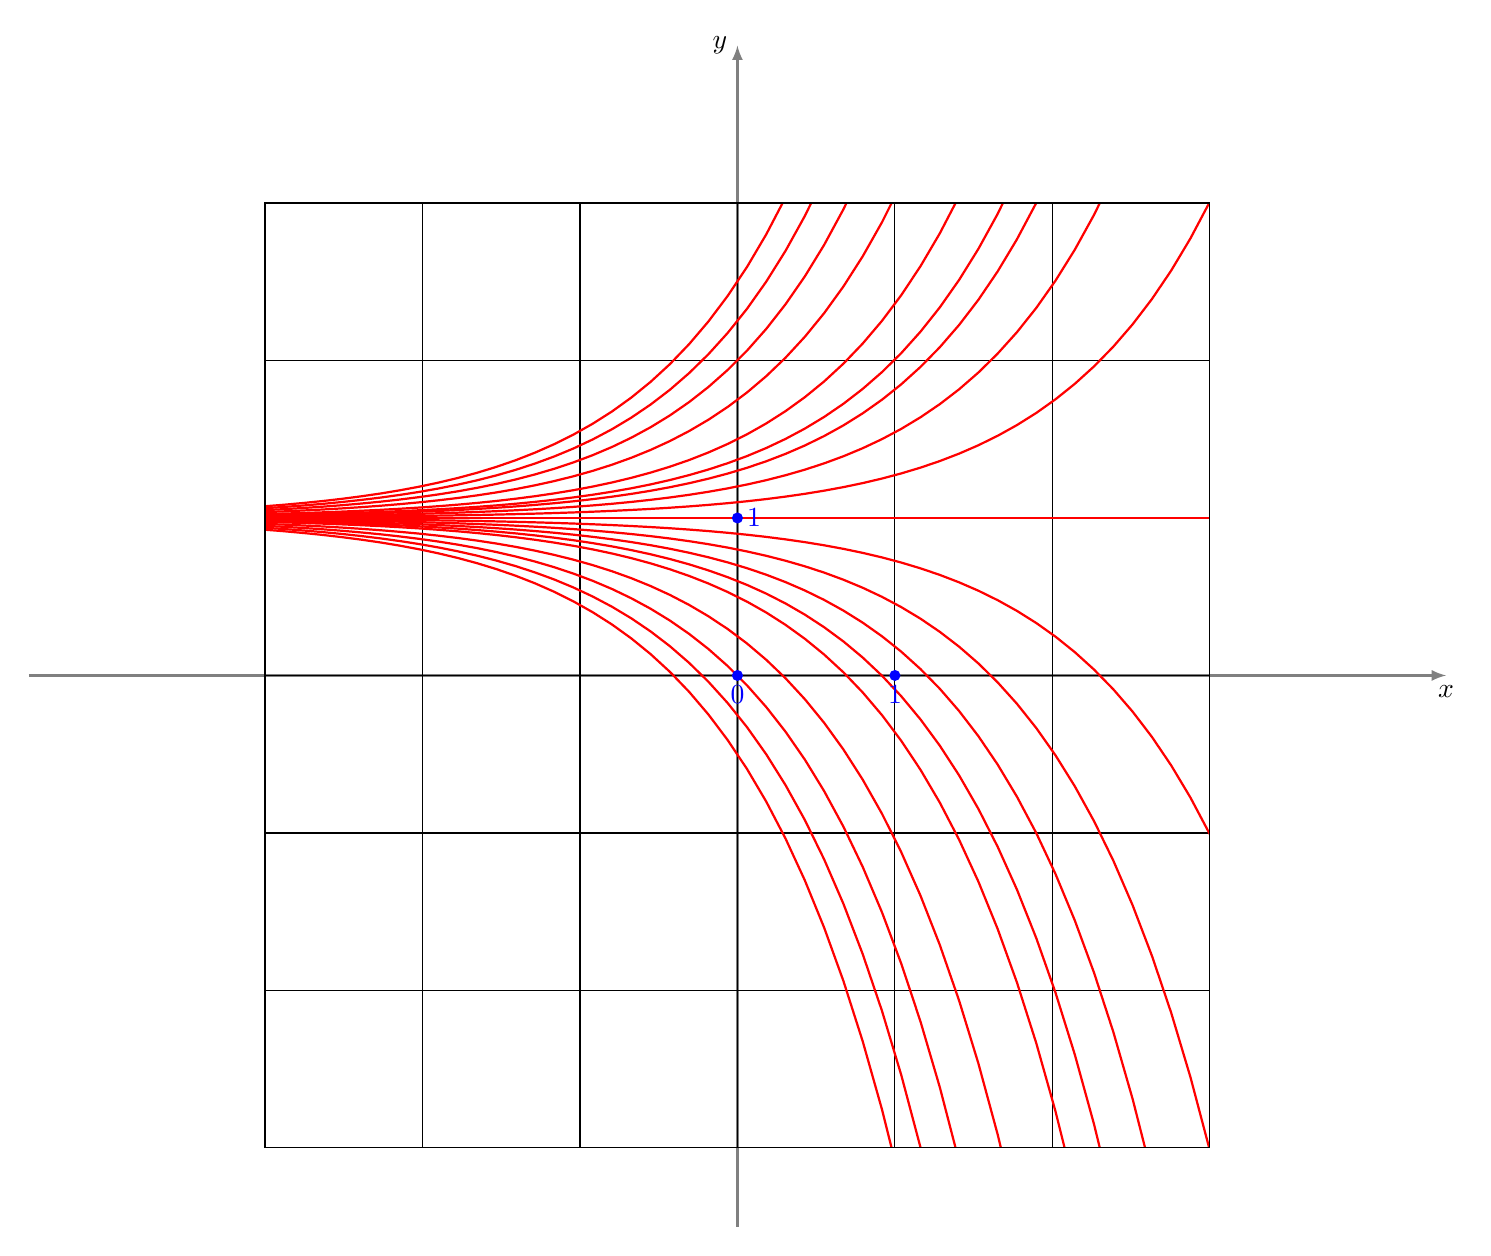
\begin{tikzpicture}[scale=2]

  \draw[->,>=latex,thick,gray] (-4.5,0) -- (4.5,0) node[below,black] {$x$};
  \draw[->,>=latex,thick,gray] (0,-3.5) -- (0,4) node[left,black] {$y$};
  \draw (-3,-3) grid (3,3);
\begin{scope}
    \clip (-3,-3) rectangle (3,3);


\foreach \k in {-1.5, -1.25,-1,-0.75,-0.5,-0.4,-0.3,-0.2,-0.1,0,0.1,0.2,0.3,0.37,0.5,0.75,1,1.25,1.5} {
  \draw[thick, color=red,domain=-3:3, samples=50] plot (\x,{\k*exp(\x)+1});
}

\end{scope}

\fill[blue] (0,0)  circle (1pt) node [below] {$0$}; 
\fill[blue] (1,0)  circle (1pt) node [below] {$1$}; 
\fill[blue] (0,1)  circle (1pt) node [right] {$1$};

\draw (-3,-3) rectangle (3,3);

\end{tikzpicture}
\end{center}


\begin{enumerate}
  \item Répondre graphiquement aux questions suivantes :
  \begin{enumerate}
    \item Quelle est la limite d'une solution en $-\infty$ ?
    \item Quelle est la solution constante ?
    \item En fonction de la valeur $f(0)$ d'une solution $f$, discuter si $f$ est croissante ou décroissante et déterminer la limite en $+\infty$.
    \item Tracer la tangente à la courbe solution qui passe par le point $(0,2)$ ; en déduire une équation approchée de cette tangente.
    \item Tracer la tangente à la courbe solution qui passe par le point $(1,-1)$ ; en déduire une équation approchée de cette tangente.
  \end{enumerate} 


  \item  Répondre par le calcul aux questions suivantes (il n'y a pas besoin de résoudre l'équation) :

  \begin{enumerate}
    \item Soit $f$ la solution dont le graphe passe par le point $(0,0)$. Combien vaut $f(0)$ ? Combien vaut $f'(0)$ ? En déduire la pente de la tangente en ce point, puis l'équation de cette tangente.

    \item  Soit $g$ la solution dont le graphe passe par le point $(1,2)$. Combien vaut $g(1)$ ? Combien vaut $g'(1)$ ? En déduire l'équation de la tangente en ce point.
  \end{enumerate} 

\end{enumerate} 
\finenonce

\indication
La pente de la tangente en $x_0$ est $f'(x_0)$.
\finindication

\correction
\sauteligne
\begin{enumerate}
  \item
  \begin{enumerate}
    \item Graphiquement on note que toutes les solutions tendent vers $1$ en $-\infty$. (Cela s'explique par le calcul, mais ce n'est pas ce qui est demandé ici.)

    \item La fonction égale à $1$ est la seule solution constante.

    \item Si $f(0)=1$, la fonction est constante égale à $1$. 
   Si $f(0)>1$, la fonction est croissante et tend vers $+\infty$ en $+\infty$.
   Si $f(0)<1$, la fonction est décroissante et tend vers $-\infty$ en $+\infty$.

    \item La tangente est tracée ci-dessous, par lecture graphique elle a pour équation $y=x+2$.

    \item La tangente est tracée ci-dessous, par lecture graphique elle a pour équation $y=-2x+1$.
  \end{enumerate} 

\begin{center}
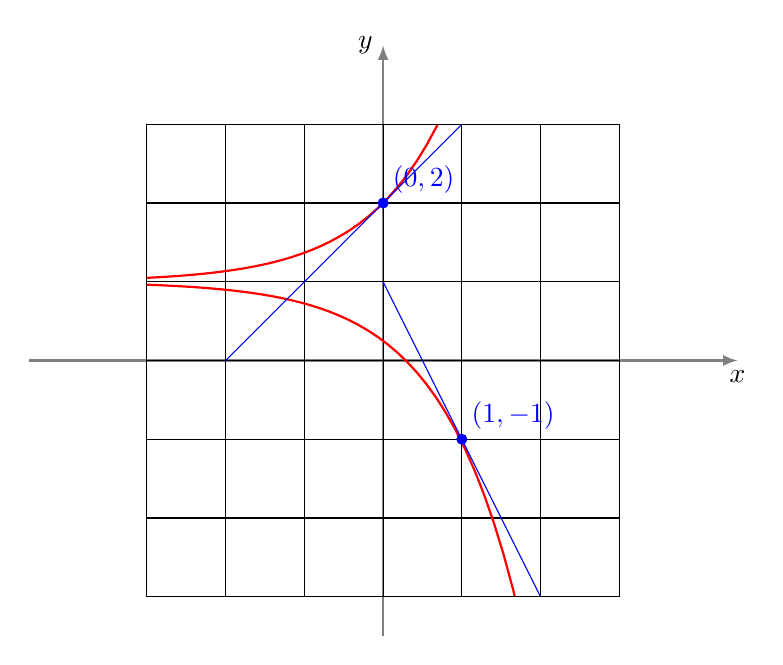
\begin{tikzpicture}[scale=1]

  \draw[->,>=latex,thick,gray] (-4.5,0) -- (4.5,0) node[below,black] {$x$};
  \draw[->,>=latex,thick,gray] (0,-3.5) -- (0,4) node[left,black] {$y$};
  \draw (-3,-3) grid (3,3);
\begin{scope}
    \clip (-3,-3) rectangle (3,3);


\foreach \k in {-0.75,1} {
  \draw[thick, color=red,domain=-3:3, samples=50] plot (\x,{\k*exp(\x)+1});
}


\fill[blue] (0,2)  circle (2pt) node[above right]{$(0,2)$};
\fill[blue] (1,-1)  circle (2pt) node[above right]{$(1,-1)$};
\end{scope}

% Tangente en (0,2)
\draw[blue] (-2,0) -- ++(3,3);

% Tangente en (1,-1)
\draw[blue] (0,1) -- ++(2,-4);

\draw (-3,-3) rectangle (3,3);

\end{tikzpicture}
\end{center}


  \item  
  \begin{enumerate}
    \item Si le graphe de $f$ passe par $(0,0)$, alors $f(0)=0$. Comme $f$ est solution de l'équation différentielle $y'=y-1$ alors pour tout $x$, $f'(x)=f(x)-1$, donc en particulier pour $x=0$ on obtient $f'(0)=f(0)-1$, donc $f'(0)=-1$.
    La pente de la tangente au graphe de $f$ en $(0,0)$ est donc $-1$. L'équation de cette tangente est donc $y=-x$ (cf graphique ci-dessous).


    \item  Si le graphe de $g$ passe par $(1,2)$, alors $g(1)=2$. Comme $g$ vérifie l'équation différentielle alors $g'(x)=g(x)-1$, donc pour $x=1$,
    $g'(1)=g(1)-1=2-1=1$. La pente de la tangente au graphe de $g$ en $(1,2)$ est donc $1$ et comme la droite passe par le point $(1,2)$, l'équation de la tangente est $y=x+1$ (cf graphique ci-dessous).
  \end{enumerate} 


\begin{center}
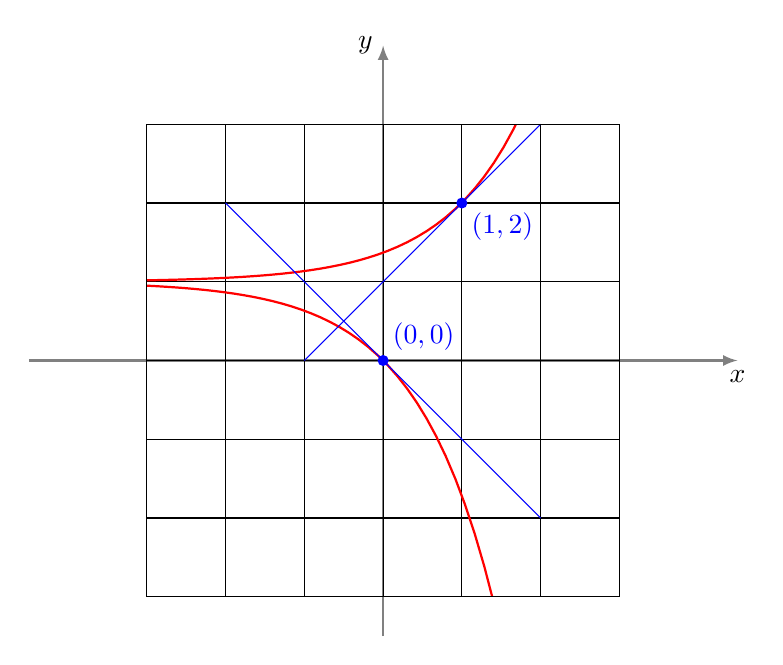
\begin{tikzpicture}[scale=1]

  \draw[->,>=latex,thick,gray] (-4.5,0) -- (4.5,0) node[below,black] {$x$};
  \draw[->,>=latex,thick,gray] (0,-3.5) -- (0,4) node[left,black] {$y$};
  \draw (-3,-3) grid (3,3);
\begin{scope}
    \clip (-3,-3) rectangle (3,3);


\foreach \k in {-1,0.37} {
  \draw[thick, color=red,domain=-3:3, samples=50] plot (\x,{\k*exp(\x)+1});
}
\fill[blue] (1,2)  circle (2pt) node[below right]{$(1,2)$}; 
\fill[blue] (0,0)  circle (2pt) node[above right]{$(0,0)$}; 

\end{scope}

% Tangente en (0,0)
\draw[blue] (-2,2) -- (2,-2);

% Tangente en (1,2)
\draw[blue] (-1,0) -- ++(3,3);

%\fill[blue] (0,0)  circle (1pt) node [below] {$0$}; 
%\fill[blue] (1,0)  circle (1pt) node [below] {$1$}; 
%\fill[blue] (0,1)  circle (1pt) node [right] {$1$};

\draw (-3,-3) rectangle (3,3);

\end{tikzpicture}
\end{center}

\end{enumerate} 
\fincorrection
\finexercice


\exercice{}
\enonce
Une tasse de café de température $T_0= 100$ degrés Celsius
est posée dans une pièce de température $T_\infty = 20$ degrés.
La loi de Newton affirme que la vitesse de décroissance de la température
est proportionnelle à l'écart entre sa température
$T(t)$ et la température ambiante $T_\infty$.

Sachant qu'au bout de $3$ minutes la température du café
est passée à $80$ degrés, quelle sera sa température au bout de $5$ minutes ?

Les questions détaillent les étapes de la résolution de ce problème :

\begin{enumerate}
  \item Justifier que la fonction température $T(t)$ satisfait l'équation différentielle 
$y' = -k(y-20)$ pour une certaine constante $k>0$.

  \item Vérifier que $T(t) = Ce^{-kt}+20$ est solution de cette équation différentielle pour toute constante $C$.

  \item Calculer $C$ en fonction de $T(0)$.

  \item Quelle est la température au bout d'un temps très long ?

  \item Déterminer la constante $k$ en utilisant que $T(3)=80$.

  \item Trouver la solution du problème.
\end{enumerate} 
\finenonce

\noindication
 
\correction
\sauteligne
\begin{enumerate}
  \item $y'$ mesure la vitesse de croissance (ou de décroissance selon le signe) de la température ; $(y-20)$ traduit l'écart entre la température du café et la température ambiante. Le coefficient $k$ exprime la proportionnalité, le signe moins venant de la décroissance de la température (le café refroidit).

  \item Pour $T(t) = Ce^{-kt}+20$, on a $T'(t) = -kCe^{-kt}$.
 Donc $-k(T(t)-20) = -k C e^{-kt} = T'(t)$ et ainsi $T(t)$ satisfait l'équation différentielle.

  \item $T(0) = Ce^{-k\cdot 0}+20 = C+20$. Comme $T(0)=100$, alors $C=80$.

  \item Comme $\lim_{t\to+\infty} Ce^{-kt} = 0$, on a $\lim_{t\to+\infty} T(t) = 20$. La température du café tendra vers $20$ degrés (c'est normal, c'est la température de la pièce).

  \item Comme $T(3)=80$ alors $80e^{-k\cdot3}+20 = 80$ donc $e^{-3k} = \frac34$.
  On compose par le logarithme des deux côtés : $\ln(e^{-3k})=\ln(\frac34)$ donc $-3k =\ln(\frac34)$ et ainsi
  $k = -\frac13\ln(\frac34) = \frac 13 \ln(\frac 43)  \simeq 0,096$. 

  \item Ainsi $T(t) \simeq 80e^{-0,096 \cdot t}+20$, donc pour $t=5$ on obtient $T(5) \simeq 80 e^{-0,096 \times 5} + 20 \simeq  69,5$ degrés Celsius.
\end{enumerate}
\fincorrection
\finexercice


\end{document}
